\chapter{Descripción de la Empresa y el Sistema}

\section{Descripción de la Empresa}

\subsection{Historia}

En 2005, el ingeniero Julio Gómez Vega comenzó a desarrollar un sistema de gestión de uniformes corporativos mientras trabajaba en la empresa textil La Scala. Tras el cierre de esta, fundó junto a Sebastián Gómez la empresa GyV Inversiones Ltda. en 2009, con el objetivo de ofrecer soluciones tecnológicas al rubro textil mediante la plataforma SISTAL.
Este sistema permitió automatizar la toma de medidas, pedidos y distribución de uniformes, consolidándose en empresas de gran tamaño como BancoEstado y Banco de Chile.
Durante más de una década, SISTAL fue una herramienta exitosa para la administración de uniformes, pero los avances tecnológicos y las nuevas exigencias en seguridad y escalabilidad motivaron su reingeniería hacia una arquitectura moderna basada en microservicios.

\subsection{Misión}

\begin{quote}
    Ser una empresa líder dentro del rubro textil, en lo que a sistemas de información se refiere, privilegiando la veracidad, rapidez y automatización de la información, con sistemas de bajo costo y fácil uso. Apostamos a la diferenciación en la comercialización mediante un servicio orientado al cliente final, con atención personalizada a cada usuario. Seremos considerados por nuestros clientes, más que un proveedor de servicios, un aliado estratégico que les ayudará a concentrarse específicamente en su negocio, dejando la administración de los uniformes corporativos en nuestras manos.
\end{quote}

\subsection{Visión}

\begin{quote}
    Formar parte de las mejores empresas de gestión de uniformes corporativos a nivel nacional e internacional, con modelos de vanguardia, una confección que cumpla con todos los estándares de calidad del mercado, y un servicio integral que exceda las expectativas de nuestros clientes. Para lograrlo, nuestro foco está apuntando a dos principios básicos, en primer lugar potenciar las fortalezas de nuestro recurso humano considerándolo como nuestro principal activo, y por supuesto, comprometernos en ir adoptando continuamente mejoras tecnológicas a nuestros sistemas informáticos.
\end{quote}

\subsection{Modelo de Negocios}

% - A que se dedica la empresa
% - principales fuentes de ingreso
% - principales catacteristicas
% - Lienzo canvas

Principales características del modelo de negocios:

\begin{itemize}
    \item Enfoque B2B (Business to Business): dirigido principalmente a empresas e instituciones que requieren gestionar la dotación de uniformes de su personal.
    \item Servicio integral: cubre todo el ciclo del proceso, desde el registro de tallas y pedidos hasta la confección y entrega de las prendas.
    \item Automatización del proceso: permite la gestión centralizada de información de usuarios, medidas y solicitudes mediante una plataforma web.
    \item Escalabilidad operativa: adaptable a distintas organizaciones, volúmenes de usuarios y flujos de trabajo.
% - Confirmar con el PO: 
    \item Modelo basado en licenciamiento y servicios: ingresos provenientes de la venta de licencias, soporte técnico y personalización del sistema.
\end{itemize}

En base al estudio realizado de la empresa, se diseñó el siguiente lienzo canvas (Figura \ref{fig:lienzo-canva-actual}).

\begin{figure}[htbp]
    \centering
    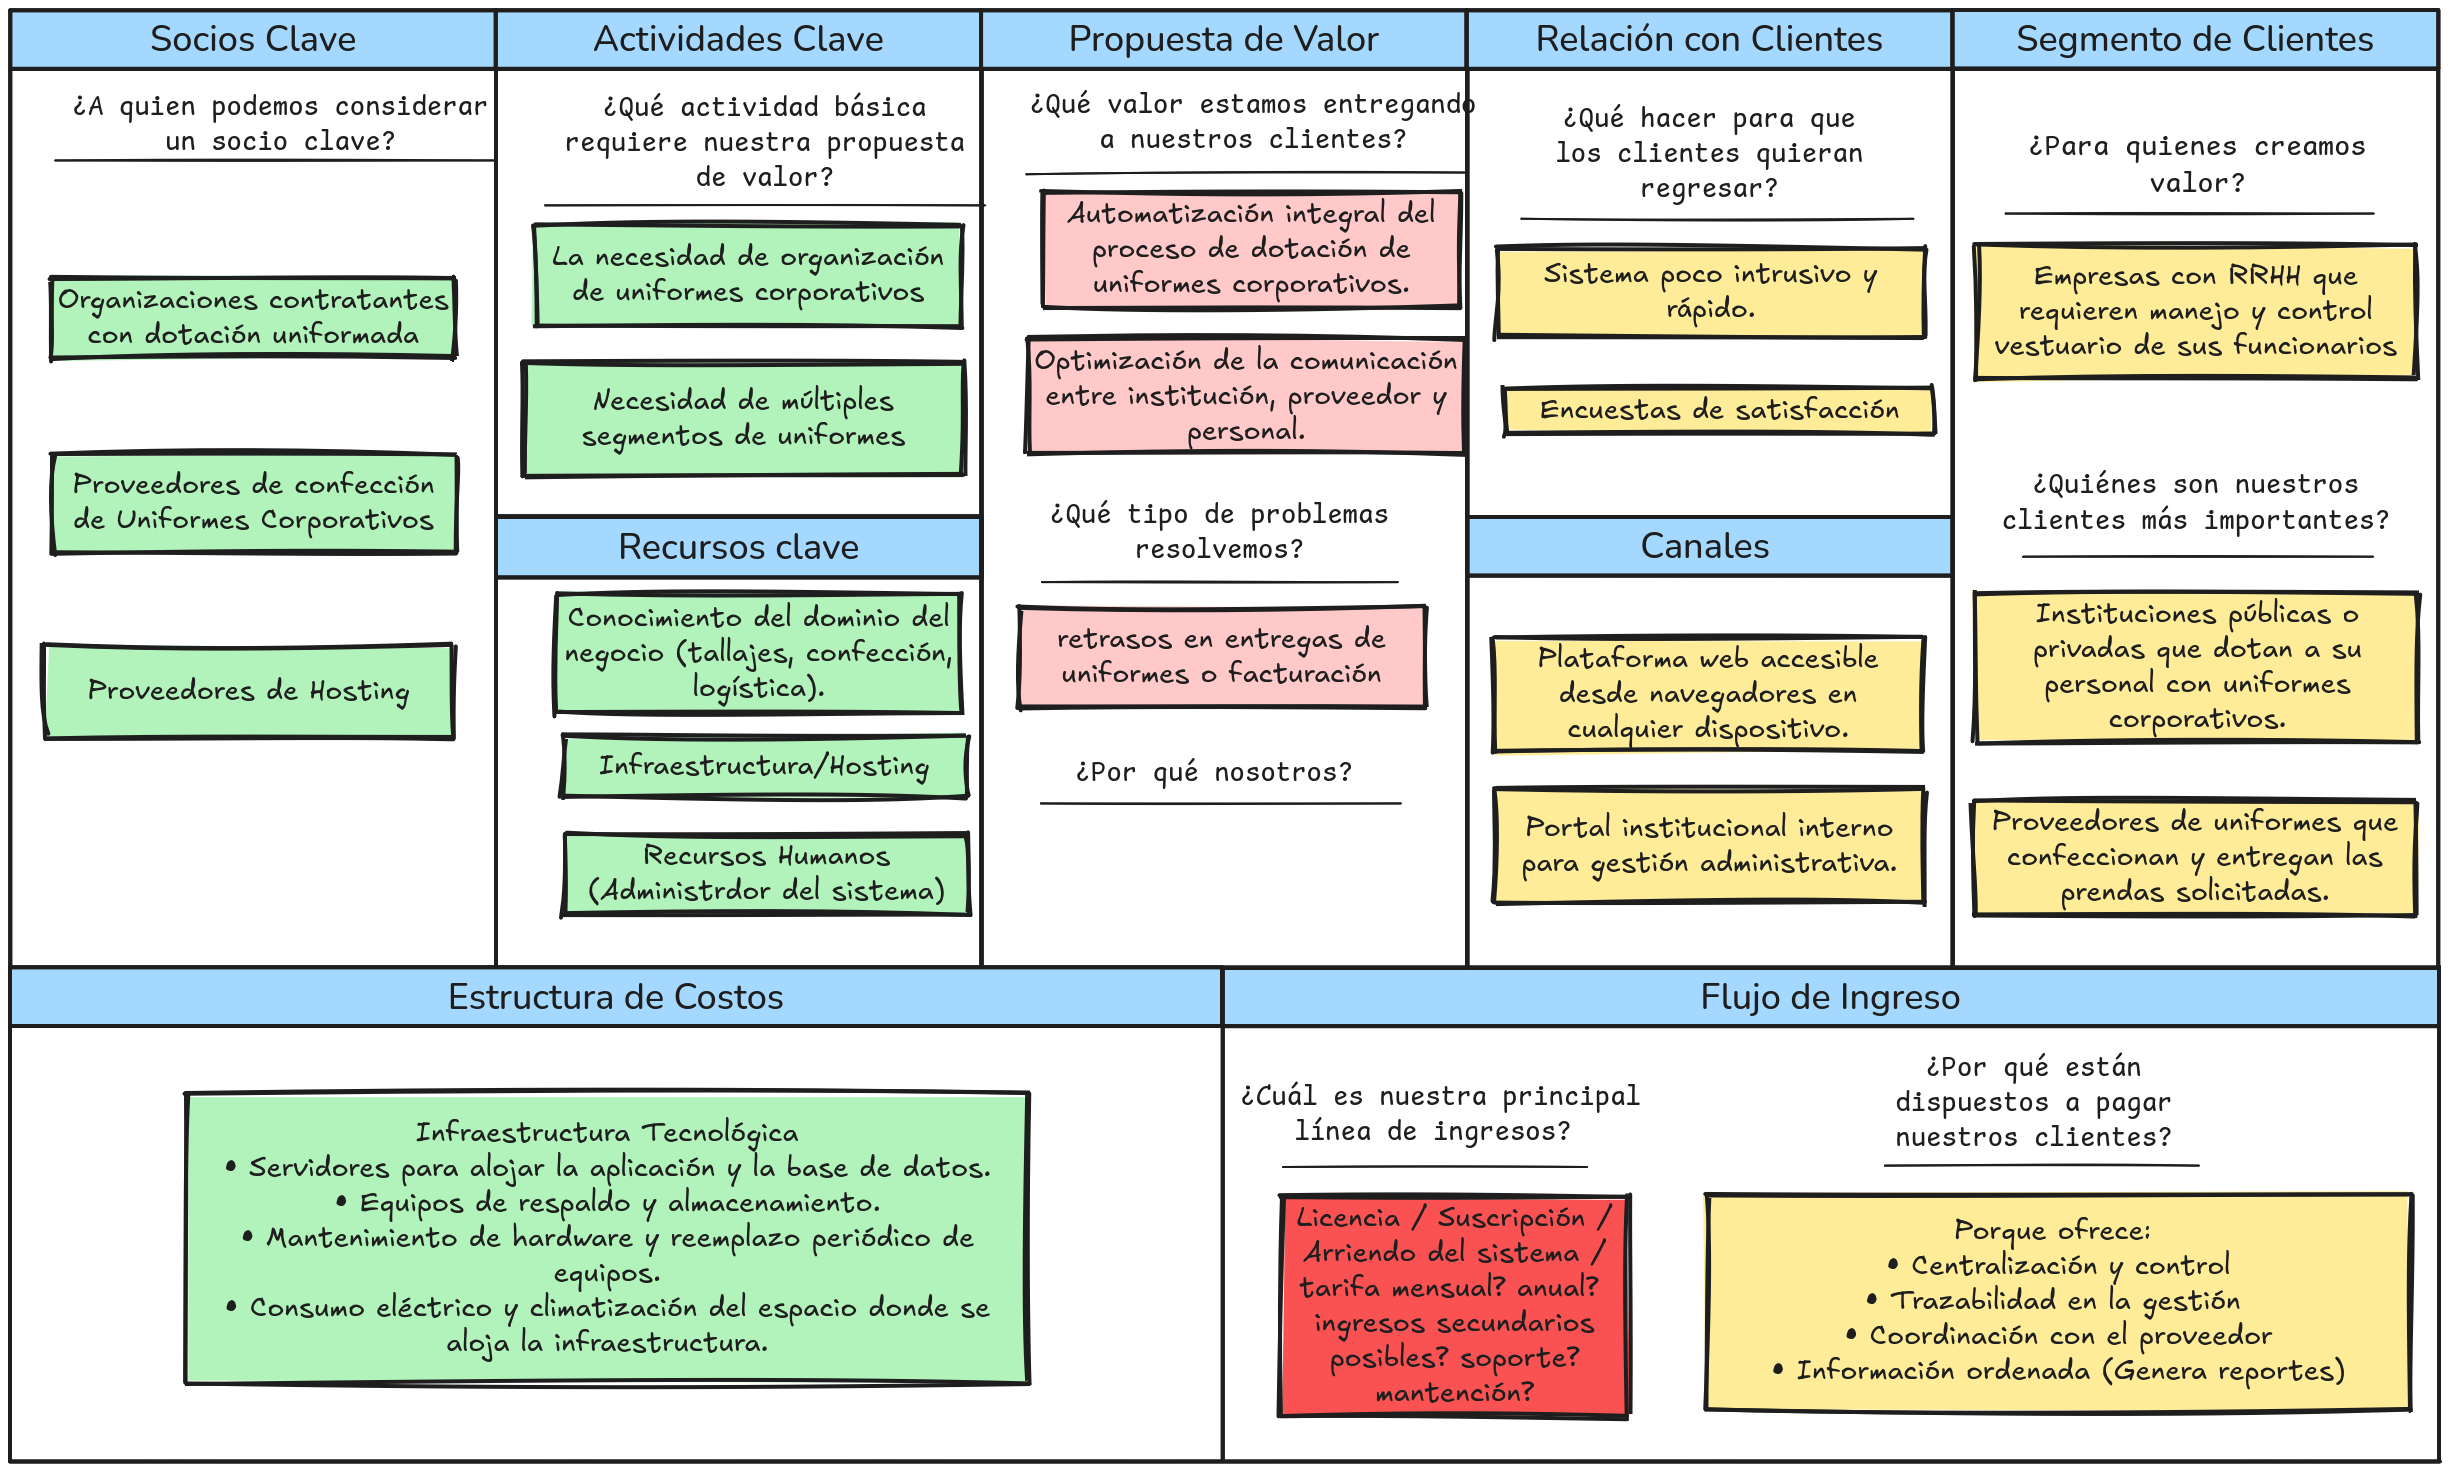
\includegraphics[width=\textwidth]{figuras/diagramas-actuales/lienzo-canva}
    \caption{Lienzo canva de la empresa actualmente}
    \label{fig:lienzo-canva-actual}
\end{figure}

\subsection{Áreas principales de la empresa}

% - descripción de las distintas áreas

\subsection{Estructura Organizacional}

% - Diagrama organizacional

\section{Descripción del Sistema (SISTAL)}

SISTAL es un sistema web de gestión de uniformes corporativos diseñado para atender a instituciones que requieren administrar de manera eficiente la dotación de prendas a su personal. La plataforma permite que cada funcionario registre sus medidas desde cualquier dispositivo con conexión a internet, información que el sistema procesa automáticamente para determinar las tallas correspondientes de cada prenda a fabricar. Posteriormente, la empresa encargada de la confección puede acceder y descargar los datos necesarios directamente desde el sistema, facilitando así la producción y el control de pedidos.

Este sistema consta de 3 actores principales en el proceso, los cuales tienen su propia vista y módulos específicos dentro del software:

\begin{itemize}
    \item \textbf{Funcionario}: Representa al usuario final perteneciente a la institución que utiliza los uniformes corporativos. Registra y actualiza sus medidas de tallaje, consulta el historial de pedidos y realiza solicitudes de cambio. El funcionario accede al sistema a través de una interfaz web desde cualquier dispositivo con conexión a internet.

    \item \textbf{Administrador (Institución)}: Actor encargado de la gestión y supervisión general del sistema. Tiene la capacidad de administrar usuarios, controlar los pedidos realizados por los funcionarios, aprobar solicitudes, generar reportes y mantener actualizada la información institucional. Además, el administrador es responsable de coordinar la comunicación entre la institución y el proveedor de uniformes, asegurando la correcta trazabilidad de los procesos y el cumplimiento de las políticas de dotación.

    \item \textbf{Proveedor (Fabricante de Uniformes)}: La empresa encargada de la confección y entrega de los uniformes. A través del sistema, el proveedor puede acceder a la información consolidada de tallas, cantidades y tipos de prendas requeridas, la cual puede descargar o consultar en línea para gestionar la producción. También puede actualizar el estado de los pedidos, registrar entregas y mantener comunicación con el administrador respecto a los plazos y disponibilidad de materiales.
\end{itemize}

\section{Objetivos}

\subsection{Objetivo General}

Diseñar la arquitectura completa del sistema de gestión de uniformes corporativos basado en microservicios en la nube, que sustituya al sistema actual y garantice mayor eficiencia operacional, escalabilidad y mantenibilidad.

% Se deberá poner esto aquí???
Como parte del proyecto, se desarrollará únicamente un módulo del sistema, a modo de implementación inicial y validación de la propuesta.


\subsection{Objetivos Específicos}

\begin{itemize}
    \item Analizar la arquitectura actual del sistema monolítico de gestión de uniformes, identificando limitaciones y oportunidades de mejora en escalabilidad y mantenibilidad.
    \item Analizar y documentar los flujos de datos a nivel de negocio con el propósito de modelarlos y replicarlos en la nueva arquitectura del sistema, asegurando su correcta adaptación y continuidad operativa en el proceso de migración.
    \item Diseñar una nueva arquitectura de microservicios escalable en la nube que permita la gestión eficiente del proceso de inventarios, pedidos, distribución y seguimiento de uniformes corporativos, considerando patrones de diseño modernos y mejores prácticas de desarrollo.
    \item Desarrollar un módulo del sistema, a modo de implementación inicial y validación de la propuesta.
\end{itemize}


\section{Alcances y Limitaciones}

\subsection{Alcances}

\begin{itemize}
    \item Reestructuración del sistema monolítico de SISTAL hacia una arquitectura de microservicios.
    \item Diseño de microservicios core para gestión de usuarios, inventarios, pedidos y estados.
    \item Configuración de infraestructura en la nube (GCP).
    \item Implementación de integración y despliegue continuo (CI/CD).
    \item Desarrollo e implementación de módulo de administración del sistema.
\end{itemize}

\subsection{Limitaciones}

\begin{itemize}
    \item No se contempla el desarrollo de aplicaciones móviles nativas o complementarias.
    \item No se usarán datos reales.
    \item No habrá capacitación masiva a usuarios finales.
    \item No se implementarán integraciones con sistemas externos no contemplados en la versión original.
    \item Se desarrollará únicamente el módulo de administración.
\end{itemize}

